\documentclass[ignorenonframetext,]{beamer}
\usetheme{Madrid}
\usecolortheme{crane}
\usepackage{amssymb,amsmath}
\usepackage{ifxetex,ifluatex}
\usepackage{fixltx2e} % provides \textsubscript
\ifxetex
  \usepackage{fontspec,xltxtra,xunicode}
  \defaultfontfeatures{Mapping=tex-text,Scale=MatchLowercase}
\else
  \ifluatex
    \usepackage{fontspec}
    \defaultfontfeatures{Mapping=tex-text,Scale=MatchLowercase}
  \else
    \usepackage[utf8]{inputenc}
  \fi
\fi
\usepackage{listings}
\usepackage{graphicx}
\makeatletter
\def\ScaleIfNeeded{%
  \ifdim\Gin@nat@width>\linewidth
    \linewidth
  \else
    \Gin@nat@width
  \fi
}
\makeatother
\let\Oldincludegraphics\includegraphics
\renewcommand{\includegraphics}[2][]{\Oldincludegraphics[width=\ScaleIfNeeded]{#2}}

% Comment these out if you don't want a slide with just the
% part/section/subsection/subsubsection title:
\AtBeginPart{
  \let\insertpartnumber\relax
  \let\partname\relax
  \frame{\partpage}
}
\AtBeginSection{
  \let\insertsectionnumber\relax
  \let\sectionname\relax
  \frame{\sectionpage}
}
\AtBeginSubsection{
  \let\insertsubsectionnumber\relax
  \let\subsectionname\relax
  \frame{\subsectionpage}
}

\setlength{\parindent}{0pt}
\setlength{\parskip}{6pt plus 2pt minus 1pt}
\setlength{\emergencystretch}{3em}  % prevent overfull lines
\setcounter{secnumdepth}{0}
\parindent=20pt
\parskip=8pt

\usepackage{ccfonts,eulervm} 
\usepackage[T1]{fontenc}
\usepackage{epigraph}
\usepackage{amsmath}
\usepackage{amsfonts}
\usepackage{amssymb}
\usepackage{fancyhdr}
\usepackage[activeacute, spanish]{babel}
\usepackage{cancel}
\usepackage[utf8]{inputenc}
\usepackage{algorithm}
\usepackage{algpseudocode}
\usepackage{afterpage}
\usepackage{url}
\usepackage{fancyhdr}

\parindent 0em
\algrenewcommand{\algorithmiccomment}[1]{//\textit{#1} }

\renewcommand{\footrulewidth}{0.4pt}
\newcommand{\hblacksquare}{\hfill \blacksquare}

\lstset{basicstyle=\footnotesize}

\title{Presentación de \emph{Paper fundacional}}
\author{A Debate on Teaching Computer Science - Dijkstra, Parnas y otros}
\date{\today}

\begin{document}
\frame{\titlepage}

\begin{frame}
\tableofcontents[hideallsubsections]
\end{frame}

\section{Introducción}

\begin{frame}\frametitle{\emph{A debate on teaching Computer Science}}

\begin{itemize}[<+->]
\itemsep1pt\parskip0pt\parsep0pt
\item
  \emph{ACM Computer Science Conference}, Febrero de 1989
\item
  Dijkstra da una charla: \emph{On the cruelty of really teaching
  computer science}
\item
  \emph{Communications of the ACM} decide publicar una carta e invita a
  un debate entre varias luminarias de las ciencias de la computación.
\item
  Uno de ellos es David Parnas.
\item
  La publicación se titula \emph{A debate on teaching Computer Science}
\end{itemize}

\end{frame}

\begin{frame}\frametitle{Dijkstra}

\begin{figure}[htbp]
\centering
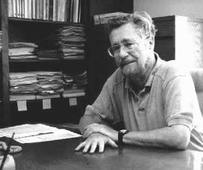
\includegraphics{dijkstra.jpg}
\caption{E. W. Dijkstra}
\end{figure}

\end{frame}

\begin{frame}\frametitle{Parnas}

\begin{figure}[htbp]
\centering
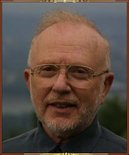
\includegraphics{parnas.jpg}
\caption{D. L. Parnas}
\end{figure}

\end{frame}

\section{On the cruelty of really teaching Computer Science}

\begin{frame}\frametitle{Reasoning by Analogy}

\begin{quote}
The underlying assumption of this talk is that computers represent a
radical novelity in our history.
\end{quote}

\begin{itemize}[<+->]
\itemsep1pt\parskip0pt\parsep0pt
\item
  Usamos analogías para trabajar con los problemas relacionados con las
  ciencias de la computación.
\item
  Queremos que los cambios sean mínimos, que nuestra experiencia sirva.
\item
  No es así con la computación\ldots{}debemos reconocer que no vale el
  sentido común.
\item
  Suprimir o ignorar la novedad: Razonamiento por analogía.

  \begin{itemize}[<+->]
  \itemsep1pt\parskip0pt\parsep0pt
  \item
    En la historia.
  \item
    En la matemática.
  \item
    En la educación.
  \end{itemize}
\item
  ¿Porqué es una novedad radical? Dos motivos: \ldots{}
\end{itemize}

\end{frame}

\begin{frame}\frametitle{Radical Novelty}

\begin{enumerate}[<+->]
\def\labelenumi{\arabic{enumi}.}
\itemsep1pt\parskip0pt\parsep0pt
\item
  Magnitud del poder de cómputo.

  \begin{itemize}[<+->]
  \itemsep1pt\parskip0pt\parsep0pt
  \item
    Complejidad muy grande gracias a la escala de cómputo.
  \item
    Jerarquías de conceptos muy profundas para esa escala.
  \item
    Única tecnología: Abarca un incomensurable espacio.
  \item
    La analogía falla: ``es como una maquina de escribir''. Error
    grosero de \emph{ratio}.
  \end{itemize}
\item
  Dispositivo digital de gran escala

  \begin{itemize}[<+->]
  \itemsep1pt\parskip0pt\parsep0pt
  \item
    Comprensión humana más ajustada a sistemas analógicos.
  \item
    Discretización produce que los comportamientos no sean
    interpolables.
  \item
    Dificulta hacer suposiciones sobre lo desconocido.
  \item
    La más mínima perturbación puede tener consecuencias drásticas.
  \item
    Negar esta novedad es serio: perdidas de millones de dolares.
  \end{itemize}
\end{enumerate}

\end{frame}

\begin{frame}\frametitle{The Doomed Discipline}

\begin{itemize}[<+->]
\itemsep1pt\parskip0pt\parsep0pt
\item
  Supersitición de ponerle nombre a algo para controlarlo.
\item
  Tratar de pensar a la computadora como cualquier dispositivo y a los
  programadores como \emph{craftsmen} ordinarios:

  \begin{itemize}[<+->]
  \itemsep1pt\parskip0pt\parsep0pt
  \item
    Medir productividad en LOC (y mal hecha la cuenta: ¡Queremos menos,
    no más!)
  \item
    Validación por \emph{testing} de programas como forma de
    pseudociencia.
  \item
    \emph{Mantenimiento de programas}: El código no se gasta\ldots{}
  \item
    Sobreenfasis en las herramientas (\emph{programmer s workbench}),
    Dijkstra las ve como infantilizantes e insipidas animaciones.
  \end{itemize}
\item
  Ingeniería de Software: \emph{snake oil business}.
\item
  Inteligencia Artificial: Emular el cerebro humano, inferior al poder
  de la máquina.
\end{itemize}

\end{frame}

\begin{frame}\frametitle{Enseñando Ciencias de la Computación}

\begin{itemize}[<+->]
\itemsep1pt\parskip0pt\parsep0pt
\item
  La computadora puede solamente manipular símbolos y mostrar resultados
  de estas derivaciones.
\item
  Un programa es un manipulador abstracto de símbolos que \emph{resulta}
  ser ejecutado en una máquina.
\item
  Manipulación de símbolos: Ciencias de la Computación como rama de la
  Lógica, a gran escala.
\item
  Visión no políticamente correcta para la academia.
\item
  Consejo de Dijkstra:

  \begin{itemize}[<+->]
  \itemsep1pt\parskip0pt\parsep0pt
  \item
    No hablar de ``bug''. Hablar de ``error''.
  \item
    No antropomorfizar la máquina:

    \begin{itemize}[<+->]
    \itemsep1pt\parskip0pt\parsep0pt
    \item
      Alejarnos de la semántica operacional.
    \item
      Razonar mediante la definición, no exhaustivamente.
    \end{itemize}
  \item
    Programación como demostración formal de teoremas.
  \item
    Evitar implementación y \emph{testing} en la enseñanza.
  \end{itemize}
\end{itemize}

\end{frame}

\section{Discusión: La respuesta de Parnas}

\begin{frame}\frametitle{La respuesta de Parnas}

\begin{itemize}[<+->]
\itemsep1pt\parskip0pt\parsep0pt
\item
  No es culpa de la Ing. del Soft. que haya malos libros.
\item
  La ingeniería no es heurística: Enfasis en validación con métodos
  formales.

  \begin{itemize}[<+->]
  \itemsep1pt\parskip0pt\parsep0pt
  \item
    Falta de profesionalismo en las ciencias de la computación.
  \end{itemize}
\item
  Hay que entender los límites de los métodos formales.

  \begin{itemize}[<+->]
  \itemsep1pt\parskip0pt\parsep0pt
  \item
    \emph{Testing} como contraejemplo a una demostración.
  \item
    Fallas en los axiomas del modelo frente a como funciona la máquina
    de verdad.
  \end{itemize}
\item
  Sensibilidad a cambios sutiles ya existe en otras disciplinas.
\item
  Para la complejidad existe \emph{Divide and Conquer} como método.
\end{itemize}

\end{frame}

\section{Nuestras conclusiones}

\begin{frame}\frametitle{Porque nos parece importante.}

\begin{itemize}[<+->]
\itemsep1pt\parskip0pt\parsep0pt
\item
  El paper nos parece fundacional o importante porque:

  \begin{itemize}[<+->]
  \itemsep1pt\parskip0pt\parsep0pt
  \item
    Enfoque novedoso a la enseñanza formal de la computación como
    ciencia.
  \item
    Podemos ver su influencia en nuestra propia carrera (ej. Algoritmos
    I y II)
  \item
    Contexto Histórico:

    \begin{itemize}[<+->]
    \itemsep1pt\parskip0pt\parsep0pt
    \item
      C++, SmallTalk. OOP gana tracción.
    \item
      Computadoras hogareñas, BASIC, Logo, aprendizaje constructivista.
    \item
      AI Winter.
    \item
      1985-1987: Therac 25.
    \end{itemize}
  \item
    Hoy mismo tenemos el problema del software.

    \begin{itemize}[<+->]
    \itemsep1pt\parskip0pt\parsep0pt
    \item
      \emph{healthcare.gov}: Un simple \emph{sitio web}, si se lo quiere
      ver así.
    \end{itemize}
  \item
    Hoy mismo esta cambiando la educación:

    \begin{itemize}[<+->]
    \itemsep1pt\parskip0pt\parsep0pt
    \item
      Treehouse, CodeAcademy, CodeSchool, Udemy, Udacity, \ldots{}
    \end{itemize}
  \end{itemize}
\end{itemize}

\end{frame}

\begin{frame}\frametitle{Nuestras conclusiones: Julián}

\begin{itemize}[<+->]
\itemsep1pt\parskip0pt\parsep0pt
\item
  Es impracticable la idea de ``approach radical novelties with a blank
  mind''.
\item
  Tampoco es practicable demostrar la correctitud de todo programa. A
  mano es difícil, con computadora es imposible (ejemplo \emph{halting
  problem}).
\item
  Tiene valor intentar simplificar los programas para hacerlos más
  fácilmente demostrables.
\item
  No todo programa tiene requerimientos tan serios: Minecraft, Angry
  Birds.
\item
  Conclusión de conclusiones: si bien en lineas generales estoy de
  acuerdo con lo que plantea Dijkstra, aplica demasiado al mundo
  académico. La computación no está acotada solo a eso.
\end{itemize}

\end{frame}

\begin{frame}\frametitle{Nuestras conclusiones: Juan Pablo}

\begin{itemize}[<+->]
\itemsep1pt\parskip0pt\parsep0pt
\item
  Ignora la aparición de Open Source y el software libre: Modelo
  colaborativo cuyo exito es difícil de explicar a nivel ingeniería del
  software.
\item
  Existe valor en la perspectiva de Dijkstra. Ejemplo: \emph{Structure
  and Interpretation of Computer Programs}.
\item
  Crítica al razonamiento por analogía y antropomorfización del software
  me parece acertado.
\item
  Las dimensiones con las que trabaja la computación siguen creciendo.
\end{itemize}

\end{frame}

\begin{frame}\frametitle{Nuestras conclusiones: Vanesa}

\begin{itemize}[<+->]
\itemsep1pt\parskip0pt\parsep0pt
\item
  A pesar de estar en desacuerdo con varios de los comentarios de
  Dijkstra
\item
  Me parece interesante y útil su crítica:

  \begin{itemize}[<+->]
  \itemsep1pt\parskip0pt\parsep0pt
  \item
    Uno se replantea el porque uno hace lo que hace y porque lo hace de
    la forma en que lo hace.
  \item
    ¿Tiene algún fundamento lo que uno hace?
  \item
    ¿Qué transmito con lo que hago, enseño o métodos que uso?
  \end{itemize}
\end{itemize}

\end{frame}

\end{document}
